%version of 09-07-19

\chapter{A graphical proof}
\label{Appendix:graphicalProof}

We are interested here in solving the problem of computing the sum of squares graphically.
\medskip

The idea here is to consider $3$ copies of the sum of squares and to reorganize them in a more simple way 
(this is Fubini's principle).
The square of $a$ is represented as $a$ copies of the unit square ()see fig.~\ref{fig:sumSquares0}).
The full process is depicted in figures Fig~\ref{fig:sumSquares1} to Fig~\ref{fig:sumSquares5}.

The height of the final rectangle is $\Delta_ n$ and its width is $2+2n-1=2n+1$. 

Thus, $3 \cdot S(n) = \Delta_n \cdot (2n+1)$, $S(n) = \frac{n(2n+1)(n+1)}{3}$.
\begin{figure}[ht]
\begin{center}
       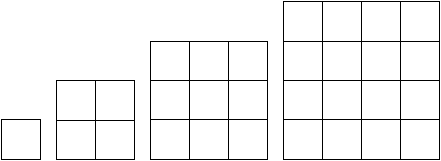
\includegraphics[scale=0.4]{FiguresMaths/SumSquares0}
\caption{Representation of the successive squares with basic unit squares.}
       \label{fig:sumSquares0}
\end{center}
\end{figure}
\begin{figure}[ht]
\begin{center}
       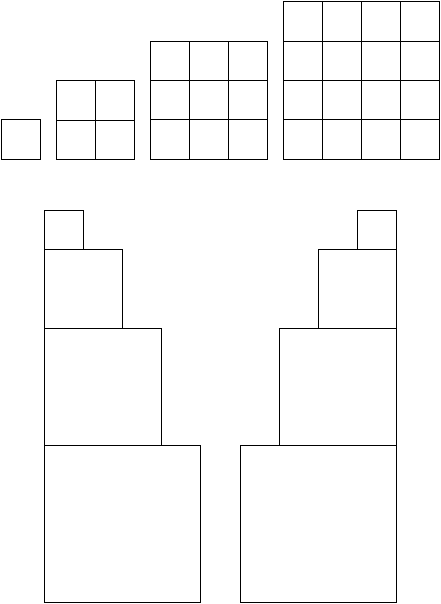
\includegraphics[scale=0.4]{FiguresMaths/SumSquares1}
\caption{Computing the sum of squares: initial configuration.}
       \label{fig:sumSquares1}
\end{center}
\end{figure}
\begin{figure}[ht]
\begin{center}
       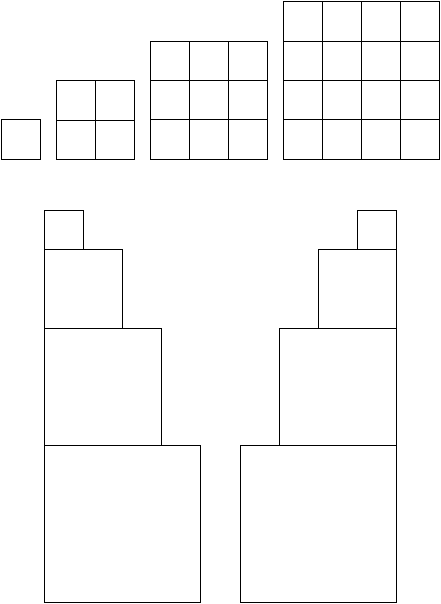
\includegraphics[scale=0.4]{FiguresMaths/SumSquares2}
\caption{Step 1 for computing the sum of squares: fill in the surface at the bottom.}
       \label{fig:sumSquares2}
\end{center}
\end{figure}
\begin{figure}[ht]
\begin{center}
       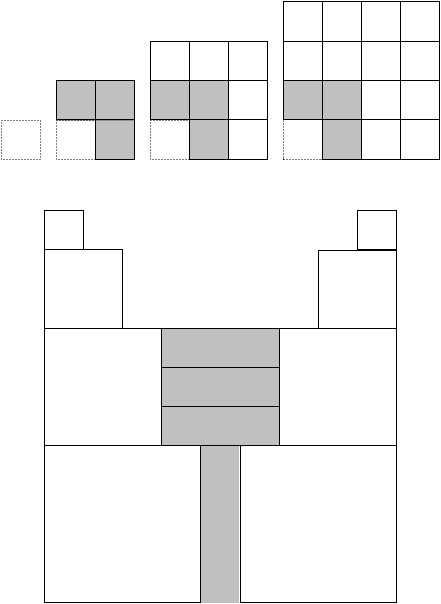
\includegraphics[scale=0.4]{FiguresMaths/SumSquares3}
\caption{Step 2 for computing the sum of squares.}
       \label{fig:sumSquares3}
\end{center}
\end{figure}
\begin{figure}[ht]
\begin{center}
       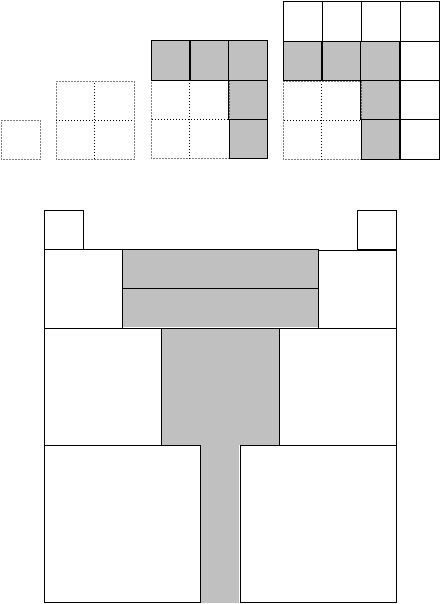
\includegraphics[scale=0.4]{FiguresMaths/SumSquares4}
\caption{Step 3 for computing the sum of squares.}
       \label{fig:sumSquares4}
\end{center}
\end{figure}
\begin{figure}[ht]
\begin{center}
       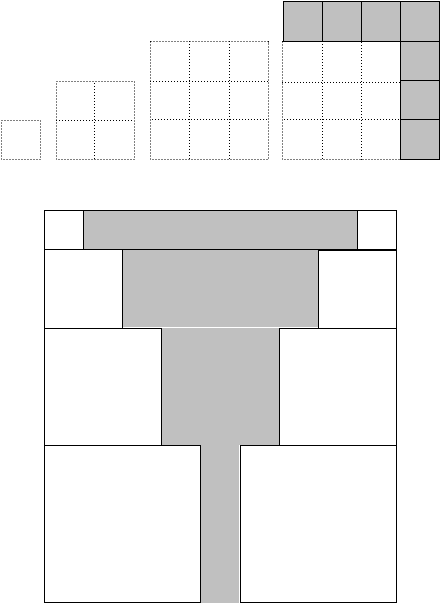
\includegraphics[scale=0.4]{FiguresMaths/SumSquares5}
\caption{Final step for computing the sum of squares: the rectangle is filled.}
       \label{fig:sumSquares5}
\end{center}
\end{figure}

